\documentclass[12pt,a4paper]{article}
\usepackage[utf8]{inputenc}
\usepackage[T1]{fontenc}
\usepackage{amsmath}
\usepackage{textcomp}

\usepackage{geometry}
\geometry{a4paper,left=25mm,right=25mm, top=2cm, bottom=2cm} 

\usepackage{graphicx} %fuer bilder

\usepackage{verbatim}




 \usepackage{mathptmx}
 \usepackage[scaled=.90]{helvet}
 \usepackage{courier}



\usepackage{listings}
\usepackage{color}
 
\definecolor{dkgreen}{rgb}{0,0.6,0}
\definecolor{gray}{rgb}{0.5,0.5,0.5}
\definecolor{mauve}{rgb}{0.58,0,0.82}

\pagestyle{empty}
\lstset{numbers=left,language=C++}
\lstset{showstringspaces=false,
basicstyle=\ttfamily\footnotesize,
breaklines=true,
tabsize=3,
commentstyle=\color{dkgreen},      % comment style
inputencoding={ansinew},
title=\lstname %zeigt titel der datei an
}

\usepackage{pdfpages} % fuer pdfs
\usepackage{hyperref} % fuer url


%keine einrückungen bei absatz
\parindent 0pt

\begin{document}
\title{Übung 02}
\author{Reinhard Penn, Bernhard Selymes}
\date{März 2015}

\normalsize

%Beginn des Dokuments

\newcommand{\Uebung}{BFMSV}
\newcommand{\srcpath}{../../src}
\newcommand{\simpath}{../../sim}

%Angabe
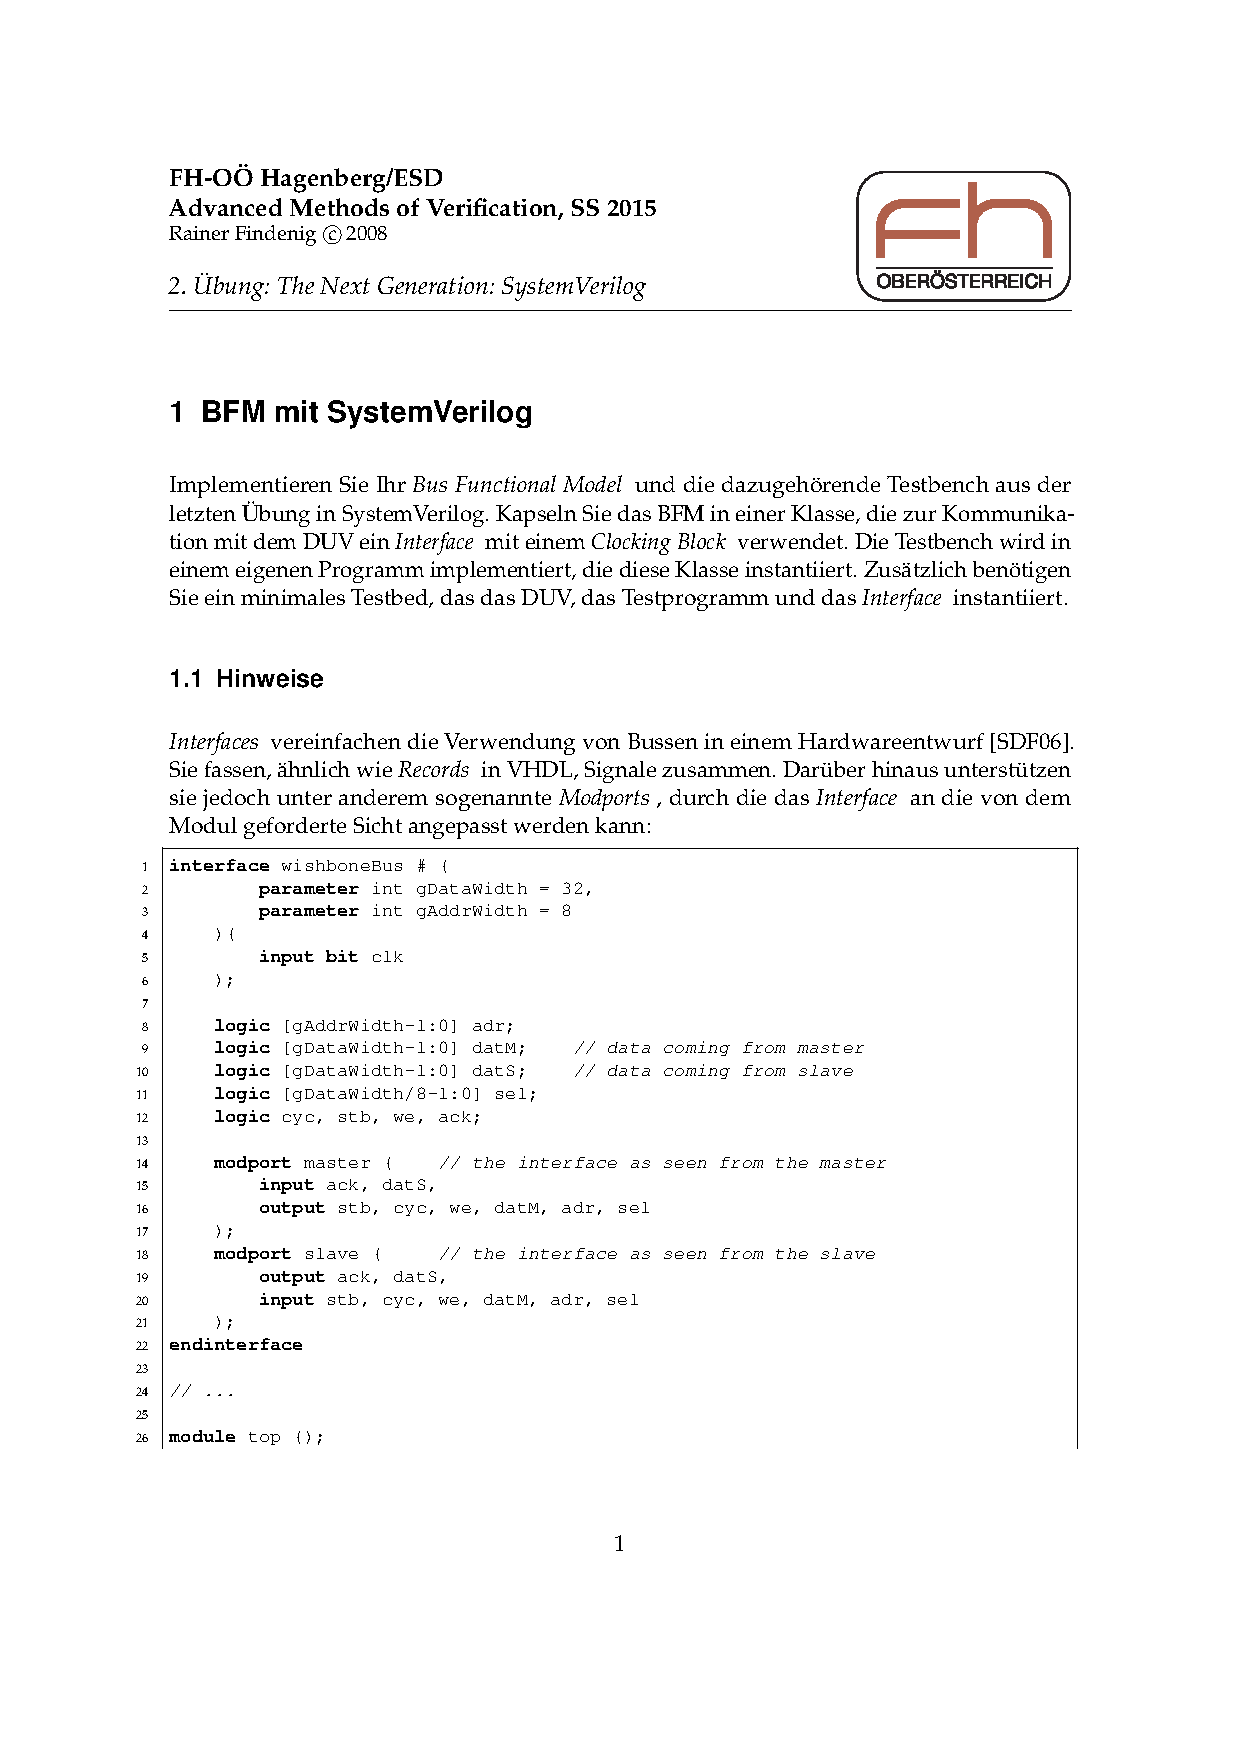
\includepdf[pages=-]{../Angabe.pdf}

\section{Beantwortung der Fragen}

\begin{itemize}
	\item \texttt{bit} ist zweiwertig und \texttt{logic} ist vierwertig. \texttt{bit} braucht weniger Speicher und \texttt{logic} ist realer.
	\item Packed vs Unpacked
		\begin{itemize}
			\item Packed Arrays sind wie Vektoren in VHDL und haben eine festgelegte Darstellung als Bit-Strom. Beispiel: \texttt{bit [7:0] inputByte}
			\item Unpacked Arrays sind wie Arrays in C, das heißt das Werkzeug kann die Abbildung frei wählen. Beispiel: \texttt{bit inputByte [7:0]}
		\end{itemize}
\end{itemize}


\section{Testfälle}
Es wurden die unten aufgelisteten Funktionen der BFM getestet. Dazu wurde der gesamte Speicherbereich des RAM zweimal geschrieben und gelesen. Beim ersten Mal waren auf der Datenleitung alle geraden Bit 1 und ungeraden Bit 0. Beim zweiten Mal wurde der Wert invertiert. 
\\
Zusätzlich gibt es noch einen Test der zur Kontrolle fehlschlagen soll und zwei Klassen die Zufallswerte zum Testen erzeugen. Die Zufallswerte werden mittels randc erzeugt.
\\
Getestet und simuliert wurde auf dem Applicationserver.

\begin{itemize}
	\item SingleRead
	\item SingleWrite
	\item BlockRead
	\item BlockWrite
\end{itemize}

\section{Source Code}

\lstinputlisting[language={verilog}]{\srcpath/wishbone_bfm.sv}

\lstinputlisting[language={tcl}]{\simpath/Compile.do}
\lstinputlisting[language={tcl}]{\simpath/Sim.do}

\end{document}
